%%================================================
%% Chapter 4
%%================================================
\chapter{ผลการดำเนินงานและอภิปรายผล}
%\label{result}
\label{chapter4}

\section{REST API สำหรับการส่งงานเขียนโปรแกรม}

\subsection{การทำงานของ API}
        \begin{figure}[H]
            \centering
                \centering
                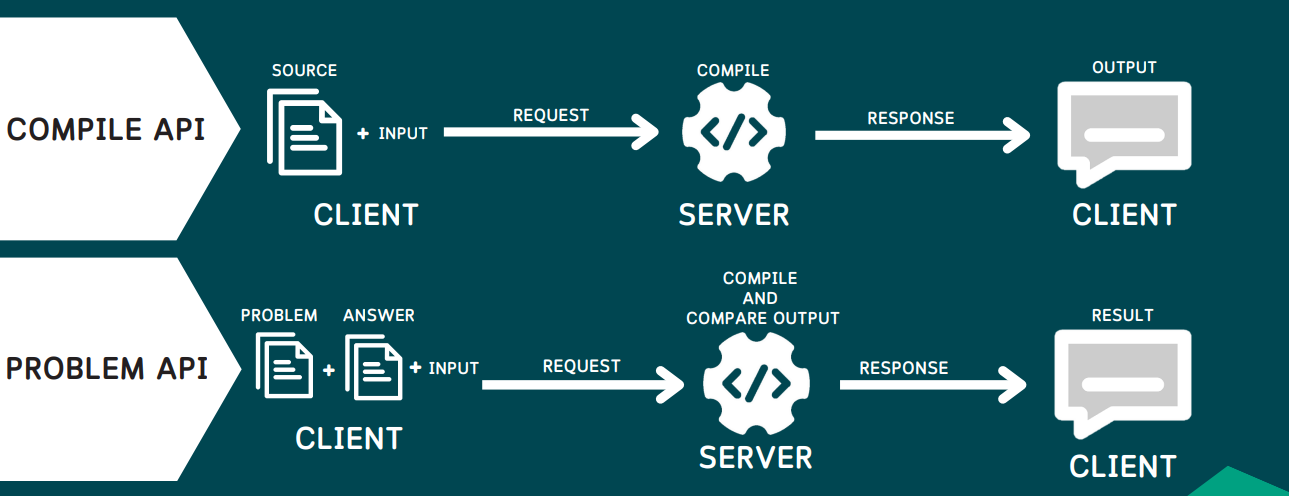
\includegraphics[width=5in]{latex/figures/api_work.png}
            \caption{การทำงานของ API}
        \end{figure}

\subsubsection{รายระเอียดการทำงานของ request API}
\begin{enumerate}
    \item compile API มีจํานวน field ทั้งหมด 3 field
        \begin{enumerate}
            \item source - ไฟล์ของโปรแกรม python หรือ java รับค่าในรูปแบบไฟล์ (source code)
            \item language - เป็นตัวบ่งชี้ว่า source code ถูกเขียนด้วยภาษาอะไร ในขณะนี้สามารถรองรับ
ภาษา python และภาษา java รับค่าในรูปแบบสตริง (string)
            \item input - ค่า input ที่จะทําการป้อนเข้าไปยัง source code รับค่าในรูปแบบสตริง (string)
        \end{enumerate}

    \item problem API มีจํานวน field ทั้งหมด 4 field
        \begin{enumerate}
            \item problem file - ไฟล์ของโจทย์ปัญหาเพื่อเอาไปเปรียบเทียบค่า output รับค่าในรูปแบบไฟล์ (source code)
            \item answer file - ไฟล์เฉลยเพื่อเอาค่า output ไปตรวจสอบความถูกต้องของ problem file รับค่าในรูปแบบไฟล์ (source code)
            \item language - เป็นตัวบ่งชี้ว่า source code ถูกเขียนด้วยภาษาอะไร ในขณะนี้สามารถรองรับ
ภาษา python และภาษา java รับค่าในรูปแบบสตริง (string)
            \item input - ค่า input ที่จะทําการป้อนเข้าไปยัง source code รับค่าในรูปแบบสตริง (string)
        \end{enumerate}
\end{enumerate}

\subsubsection{ตัวอย่างการเรียกใช้งาน API}
\begin{enumerate}
    \item ตัวอย่างการเรียกใช้ compile API
    \begin{enumerate}
            \item URL คือ http://localhost:8081/compile
            \item Request body
                \begin{enumerate}
                    \item source
                    \item language
                    \item input
                \end{enumerate}
            \item response
                \begin{enumerate}
                    \item output
                \end{enumerate}
        \end{enumerate}

    \begin{figure}[H]
            \centering
                \centering
                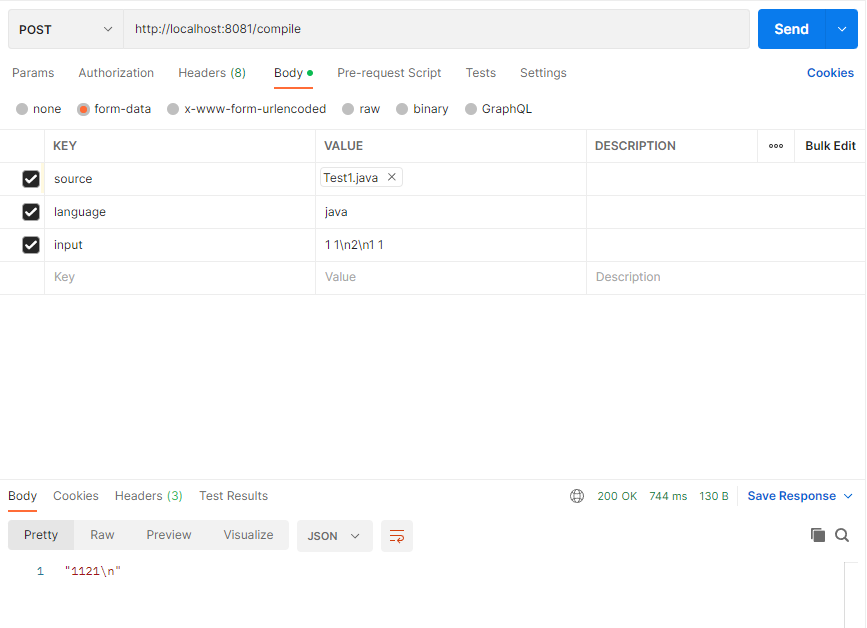
\includegraphics[width=5in]{latex/figures/compilepost.png}
            \caption{ตัวอย่างการใช้ compile API}
    \end{figure}

    \item ตัวอย่างการเรียกใช้ problem API
    \begin{enumerate}
            \item URL คือ http://localhost:8081/problem
            \item Request body
                \begin{enumerate}
                    \item problem file
                    \item answer file
                    \item language
                    \item input
                \end{enumerate}
            \item response
                \begin{enumerate}
                    \item output
                \end{enumerate}
        \end{enumerate}

    \begin{figure}[H]
            \centering
                \centering
                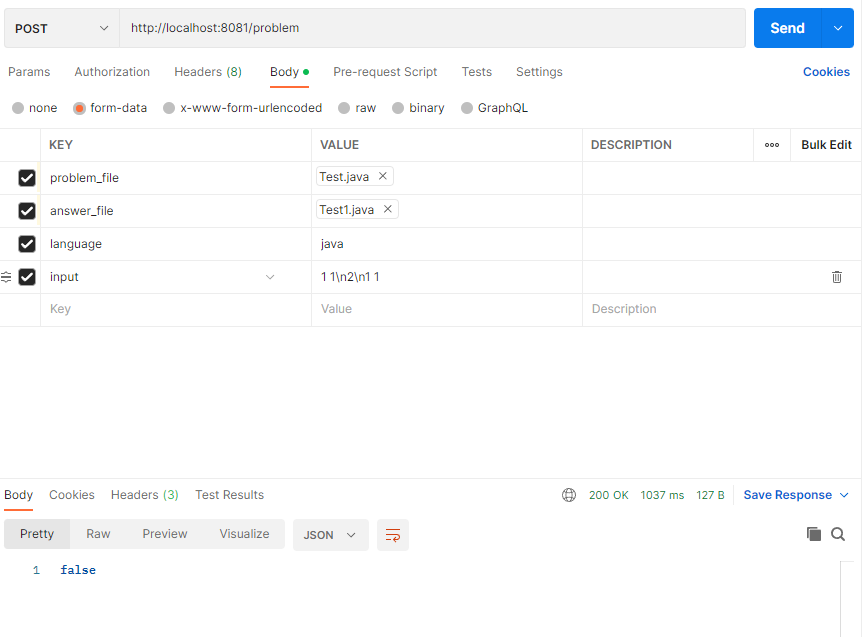
\includegraphics[width=5in]{latex/figures/problempost.png}
            \caption{ตัวอย่างการใช้ problem API}
    \end{figure}
\end{enumerate}

\section{คำอธิบายของ API}
การที่ทำ API ให้ผู้ใช้งานสามารถเข้าใจได้ว่า API นั้นไว้ทำอะไรและใช้อย่างไร โดยมีมาตราฐานของการอธิบายอยู่คือ OpenAPI
        \begin{figure}[H]
            \centering
                \centering
                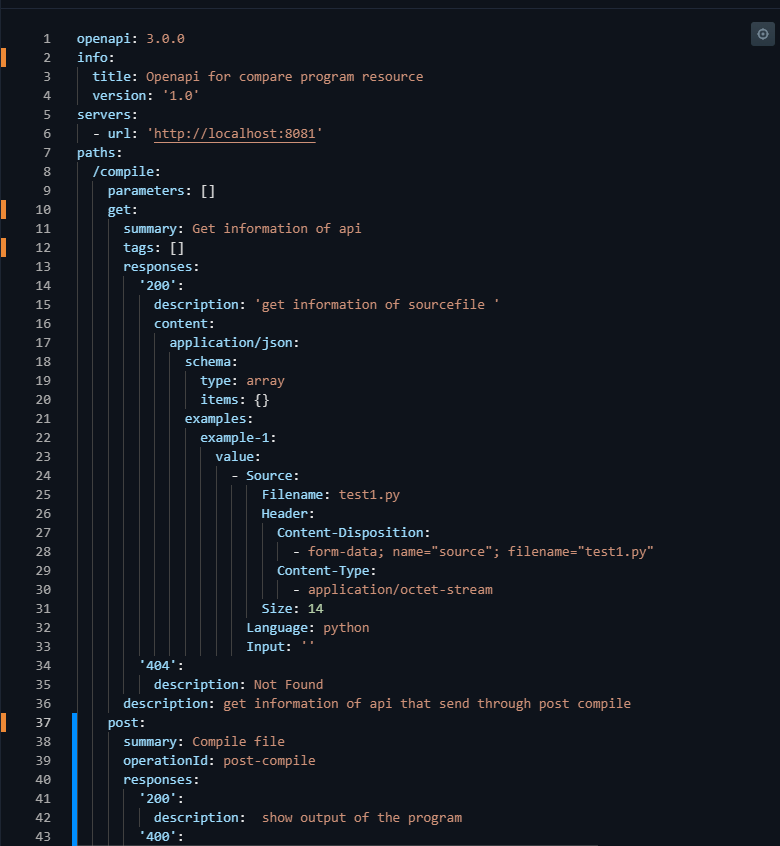
\includegraphics[width=5in]{latex/figures/OAS.png}
            \caption{OpenAPI Specification}
        \end{figure}
\section{deploy ลง docker}
ผู้จัดทำเลือก deploy ลง docker เพื่อให้ทดสอบการให้ทำงานเปรียบเสมือนเครื่อง server ที่จะสามารถทดสอบการใช้งานจริงได้ 
\begin{figure}[H]
    \centering
        \centering
        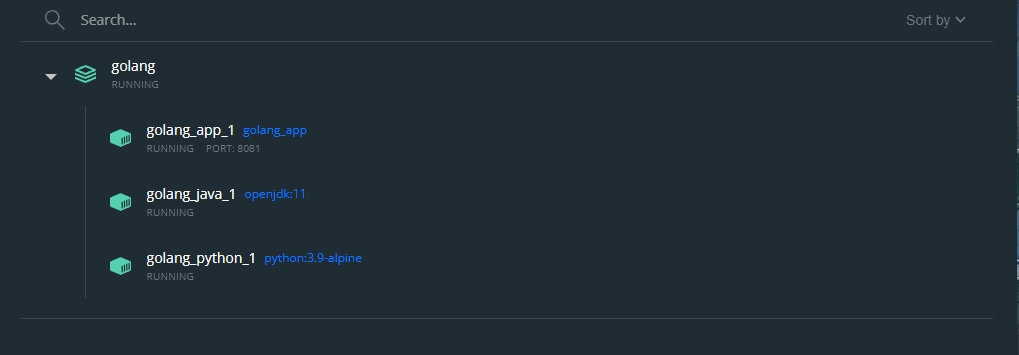
\includegraphics[width=5in]{latex/figures/docker.png}
    \caption{docker container}
\end{figure}

\section{เว็บตัวอย่าง}
ทำการสร้างเว็บตัวอย่างเพื่อทดสอบการใช้งานจริงโดยเรียกใช้ compile API และ problem API โดยเลือกส่ง API request ไปที่ server (docker) ที่ได้จัดเตรียมไว้
    \begin{figure}[H]
        \centering
            \centering
            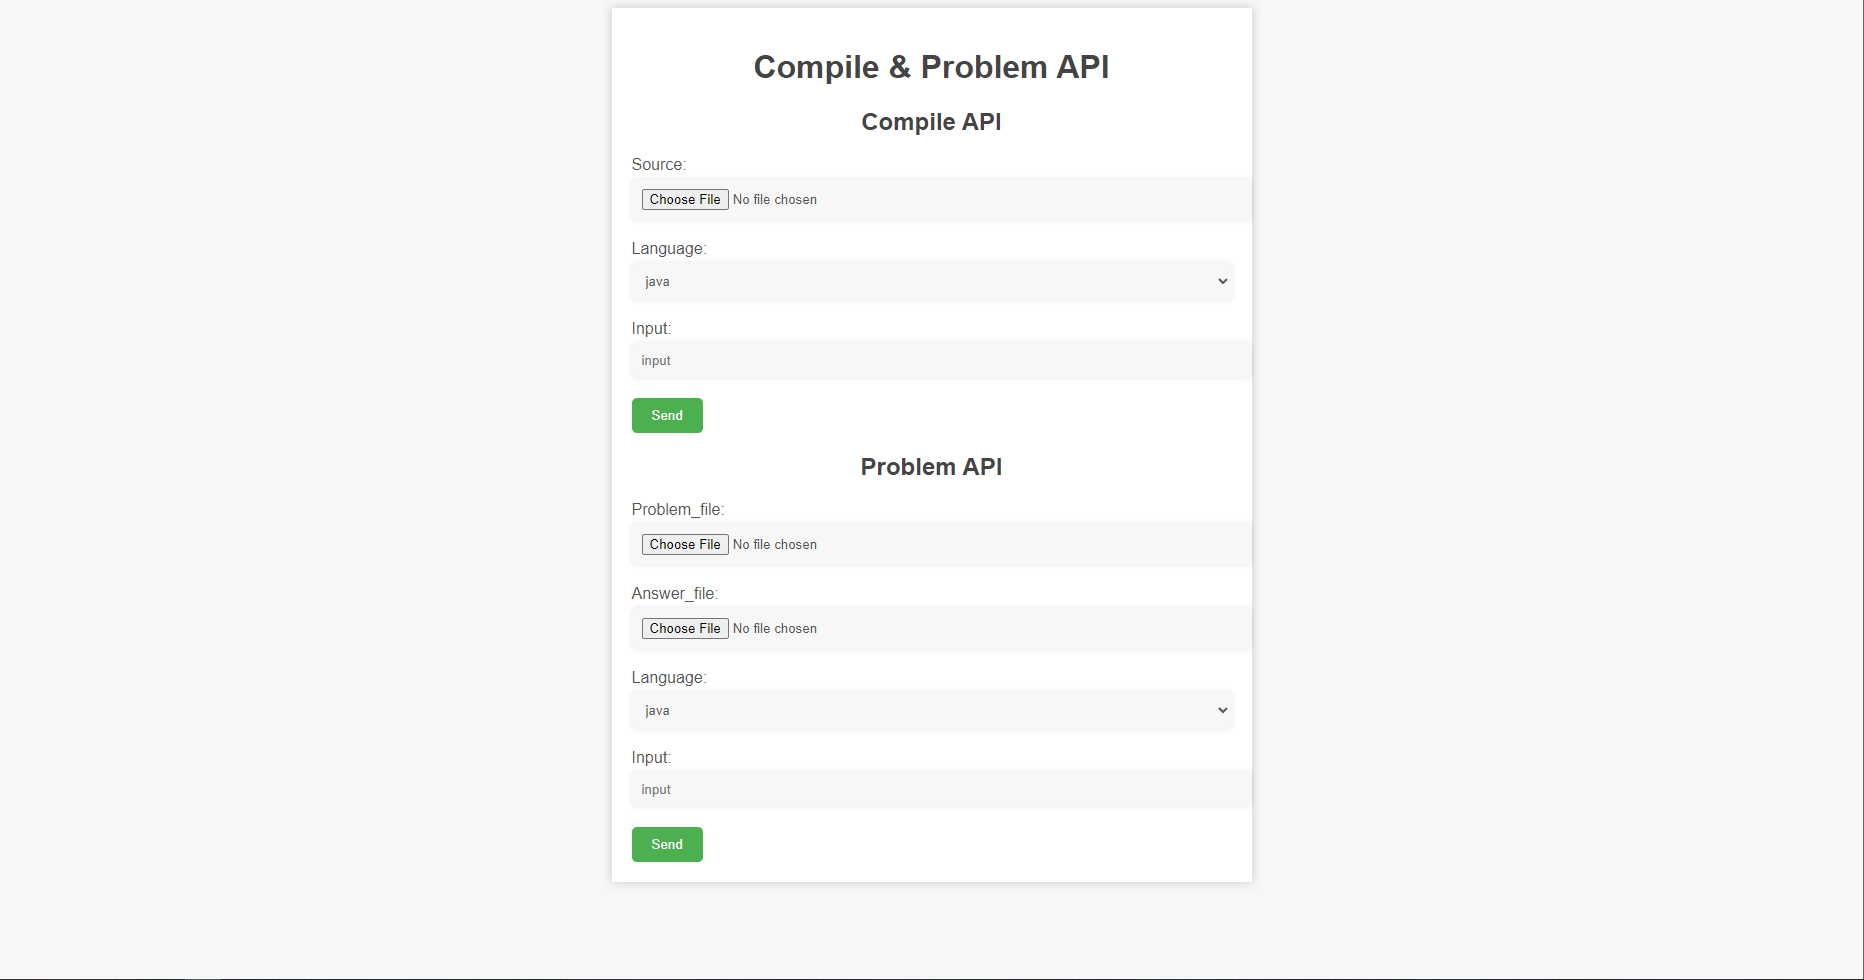
\includegraphics[width=5in]{latex/figures/web.png}
        \caption{ตัวอย่างหน้าเว็บ}
    \end{figure}

